

\tikzset{every picture/.style={line width=0.75pt}} %set default line width to 0.75pt        

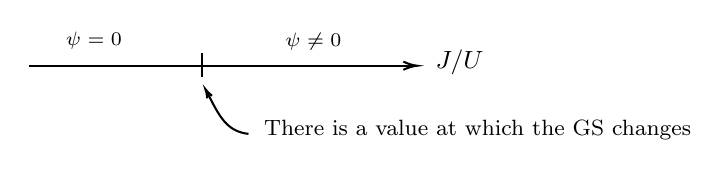
\begin{tikzpicture}[x=0.75pt,y=0.75pt,yscale=-1,xscale=1]
%uncomment if require: \path (0,75); %set diagram left start at 0, and has height of 75

%Straight Lines [id:da7677509231373215] 
\draw    (10.5,26.86) -- (195.57,26.86) ;
\draw [shift={(197.57,26.86)}, rotate = 180] [color={rgb, 255:red, 0; green, 0; blue, 0 }  ][line width=0.75]    (6.56,-1.97) .. controls (4.17,-0.84) and (1.99,-0.18) .. (0,0) .. controls (1.99,0.18) and (4.17,0.84) .. (6.56,1.97)   ;
%Straight Lines [id:da3257796010864502] 
\draw    (94,20.9) -- (94,32.1) ;
%Curve Lines [id:da5122812185238221] 
\draw    (116.4,59.7) .. controls (105.38,58.56) and (101.94,50.2) .. (96.48,39.76) ;
\draw [shift={(95.6,38.1)}, rotate = 61.82] [color={rgb, 255:red, 0; green, 0; blue, 0 }  ][line width=0.75]    (4.37,-1.32) .. controls (2.78,-0.56) and (1.32,-0.12) .. (0,0) .. controls (1.32,0.12) and (2.78,0.56) .. (4.37,1.32)   ;

% Text Node
\draw (205,17.63) node [anchor=north west][inner sep=0.75pt]  [font=\small]  {$J/U$};
% Text Node
\draw (26.91,9.03) node [anchor=north west][inner sep=0.75pt]  [font=\scriptsize]  {$\psi =0$};
% Text Node
\draw (132.71,9.43) node [anchor=north west][inner sep=0.75pt]  [font=\scriptsize]  {$\psi \neq 0$};
% Text Node
\draw (122.4,51.8) node [anchor=north west][inner sep=0.75pt]  [font=\footnotesize] [align=left] {There is a value at which the GS changes};


\end{tikzpicture}
